\section{Principali tecniche di heap exploitation}
Nell'uso di \verb+malloc+ e \verb+free+ è responsabilità del programmatore:
\begin{enumerate}
	\item liberare una zona di memoria con \verb+free+ ottenuta da \verb+malloc+\label{reg:free-no-malloc}\footnote{e funzioni \verb+malloc+ compatibili, come \verb+calloc+, \verb+realloc+ e \verb+memalign+.}
	\item non usare \verb+free+ su una zona di memoria più di una volta\label{reg:free2}
	\item assicurarsi di non sovrascrivere zone di memoria che eccedono la memoria richiesta con \verb+malloc+, per evitare \emph{heap overflow}\label{reg:overflow}
\end{enumerate}

Non rispettando queste regole è possibile sfruttare le vulnerabilità presenti in un programma per eseguire codice arbitrario. Gli Shellphish, un famoso gruppo di Capture The Flag (CTF), hanno elencato una serie di possibili attacchi nel repository Github \emph{how2heap}\cite{how2heap}.

La Tabella~\ref{tab:heap-att} mostra una lista di possibili attacchi che sfruttano alcune vulnerabilità presenti nel codice.

\begin{table}
	\centering
	\begin{tabular}{lll}
		Nome dell'attacco & Tecnica \\
		\midrule
		Fastbin dup & Indurre la \texttt{malloc} a restituire un chunk in heap già allocato sfruttando i fastbin \\
		Fastbin dup into stack & Indurre la \texttt{malloc} a restituire un puntatore arbitrario sfruttando i fastbin \\
		Fastbin dup consolidate & Indurre la \texttt{malloc} a restituire un chunk in heap già allocato,\\
		& inserendo il puntatore in un fastbin e nell'unsorted bin \\
		Unsafe unlink & Utilizzare la \texttt{free} su un fake chunk per ottenere un \emph{arbitrary write} \\
		House of spirit & Utilizzare la \texttt{free} su un fake chunk per avere un puntatore ad un chunk aribitrario \\
		House of lore & Indurre la \texttt{malloc} a restituire un puntatore aribitrario sfruttando uno smallbin \\
		House of force & Sfruttare l'header del \emph{top chunk} per avere un puntatore arbitrario \\
		House of orange & Sfruttare il \emph{top chunk} per ottenere \emph{arbitrary code execution} \\
		Large bin attack & Sfruttare un chunk libero in un large bin per ottenere un \emph{arbitrary write} \\
		\bottomrule
	\end{tabular}
	\vspace{0.15in}
	\caption{Lista dei principali attacchi su heap (fonte~\cite{how2heap})}
	\label{tab:heap-att}
\end{table}

In questa trattazione, in particolare, vedremo in dettaglio quattro di questi attacchi: \emph{fastbin dup}, \emph{fastbin dup into stack}, \emph{unsafe unlink} e \emph{house of spirit}.

\subsection{Fastbin dup}\label{cap:fastbin-dup}
\emph{Fastbin dup} permette di ottenere da una \verb+malloc+ un chunk di memoria già allocato precedentemente, sfruttando i fastbin.

Vediamo l'attacco. Si inizia allocando inizialmente tre buffer con una dimensione che entri in un fastbin:
\begin{lstlisting}[style=CStyle]
int *a = malloc(8);
int *b = malloc(8);
int *c = malloc(8);
\end{lstlisting}

Rilasciamo \verb+a+:
\begin{lstlisting}[style=CStyle]
free(a);
\end{lstlisting}

A questo punto, \verb+a+ contiene ancora il puntatore del chunk di memoria in heap che ora è libero.
Se invocassimo nuovamente \verb+free(a)+, essa si accorgerebbe che \verb+a+ è già stato liberato poichè si trova in testa a \verb+fastbin[0]+\footnote{Si noti che \verb+free+ in questo caso non può controllare il bit \verb+prev_inuse+ del chunk successivo in memoria poichè, come già detto nel precedente capitolo, in un fastbin i chunk non sono liberati effettivamente}.
Ispezionando il codice nella libc della \verb+free+ si può notare come questa faccia proprio questo controllo:
\begin{lstlisting}[style=CStyle]
/* Check that the top of the bin is not the record we are going to add
    (i.e., double free).  */
 if (__builtin_expect (old == p, 0))
   {
     errstr = "double free or corruption (fasttop)";
     goto errout;
   }
\end{lstlisting}
dove \verb+old+ è un puntatore al primo elemento del fastbin selezionato e \verb+p+ è il puntatore al chunk passato alla \verb+free+.

Per questo si invoca la \verb+free+ prima sul puntatore \verb+b+:
\begin{lstlisting}[style=CStyle]
free(b);
\end{lstlisting}
per poi invocarla nuovamente su \verb+a+:
\begin{lstlisting}[style=CStyle]
free(a);
\end{lstlisting}

\verb+fastbin[0]+ contiene ora questi puntatori: \verb+[a, b, a]+\footnote{con un abuso di notazione in quanto i puntatori restituiti dalla \verb+malloc+ non sono gli stessi dei chunk su cui opera invece la \verb+free+}.

Richiamando tre \verb+malloc+ consecutive:
\begin{lstlisting}[style=CStyle]
fprintf(stdout, "1st malloc(8): %p\n", malloc(8));
fprintf(stdout, "2nd malloc(8): %p\n", malloc(8));
fprintf(stdout, "3rd malloc(8): %p\n", malloc(8));
\end{lstlisting}
la prima e la terza \verb+malloc+ restituiranno lo stesso puntatore.

Da notare come questo bug è stato ottenuto poichè si è violata la regola~\ref{reg:free2}.

\subsection{Fastbin dup into stack}
\emph{Fastbin dup into stack} permette di ottenere un puntatore ad una zona in memoria arbitraria sfruttando, come in \emph{fastbin dup} (vedi Paragrafo~\ref{cap:fastbin-dup}), un fastbin.

Il prologo è lo stesso di \emph{fastbin dup}:
\begin{lstlisting}[style=CStyle]
int *a = malloc(8);
int *b = malloc(8);
int *c = malloc(8);

free(a);
free(b);
free(a);
\end{lstlisting}
in modo che \verb+fastbin[0]+ contenga la lista \verb+[a, b, a]+.

Si definisce inoltre una variabile \verb+stack_var+:
\begin{lstlisting}[style=CStyle]
uint64_t stack_var;
\end{lstlisting}

Eseguendo una \verb+malloc+:
\begin{lstlisting}[style=CStyle]
int *d = malloc(8);
\end{lstlisting}

\verb+d+ contiene il puntatore ad \verb+a+\footnote{inteso come locazione in memoria, e non come puntatore alla variabile \verb+a+}.

Eseguendo nuovamente \verb+malloc(8)+, \verb+fastbin[0]+ conterrà \verb+[a]+, quindi se sovrascriviamo \verb+d+, sovrascriviamo anche \verb+a+ essendo lo stesso puntatore.

Sovrascriviamo quindi \verb+d+ con
\begin{lstlisting}[style=CStyle]
*d = (uint64_t) (((char*)&stack_var) - sizeof(d));
\end{lstlisting}
modificando nello stesso tempo anche il campo \verb+fd+ di \verb+a+.

Poichè la \verb+malloc+ effettua un controllo sulla \verb+size+ del chunk puntato da \verb+fd+, si assegna a \verb+stack_var+ la dimensione dei chunk contenuti nel \verb+fastbin[0]+:
\begin{lstlisting}[style=CStyle]
stack_var = 0x20;
\end{lstlisting}

Con \verb+malloc(8)+ si estrae da \verb+fastbin[0]+ il chunk \verb+a+, e poichè \verb+a->fd != NULL+, si inserisce in testa a \verb+fastbin[0]+ il puntatore \verb+a->fd+.
L'ultima \verb+malloc(8)+ ci consente di ottenere l'indirizzo scelto, in questo caso \verb|(char*)&stack_var + 8|.

In questo esempio si è scelto l'indirizzo di una variabile in stack come puntatore restituito da \verb+malloc+,  ma è possibile scegliere qualsiasi altro indirizzo: nella CTF presentata nel Paragrafo~\ref{cap:babyheap} l'indirizzo scelto è infatti una entry della \verb+.got+.


\subsection{Unsafe unlink}
\emph{Unsafe unlink} consente di ottenere un \emph{arbitrary write} utilizzando la \verb+free+ per corrompere un chunk libero. Lo scenario di utilizzo di questo attacco prevede la presenza di un puntatore globale ad un buffer su cui si può fare overflow.

Sia \verb+malloc_size = 0x80+ una variabile contente la dimensione di un chunk maggiore di un fastbin.
Sia \verb+chunk0_ptr+ un puntatore globale, che punta ad un buffer di dimensione \verb+malloc_size+, ottenuto da una \verb+malloc+.
Sia \verb+chunk1_ptr+ il puntatore ad un buffer di dimensione \verb+malloc_size+, ottenuto anch'esso da una \verb+malloc+.

\begin{lstlisting}[style=CStyle]
chunk0_ptr = malloc(malloc_size);            //chunk0
uint64_t *chunk1_ptr = malloc(malloc_size);  //chunk1
\end{lstlisting}

Si crea un fake chunk all'interno di \verb+chunk0+, in modo tale che l'\verb+unlink+, una funzione utilizzata dalla \verb+free+ per rimuovere un elemento da un bin, possa superare il controllo \verb+P->fd->bk == P && P->bk->fd == P+ (vedi Figura~\ref{fig:unlink}):

\begin{figure}
	\centering
	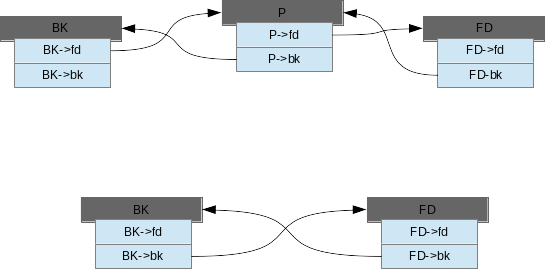
\includegraphics[width=7cm]{unlink}
	\caption{Rimozione del chunk P dall'\texttt{unlink}}
	\label{fig:unlink}
\end{figure}

\begin{lstlisting}[style=CStyle]
chunk0_ptr[2] = (uint64_t) &chunk0_ptr-(sizeof(uint64_t)*3);
chunk0_ptr[3] = (uint64_t) &chunk0_ptr-(sizeof(uint64_t)*2);
\end{lstlisting}

Si ottiene una situazione illustrata nella Figura~\ref{fig:unsafe_unlink1}.

\begin{figure}
	\centering
	\includegraphics[width=10cm]{unsafe_unlink1}
	\caption{Creazione del fake chunk}
	\label{fig:unsafe_unlink1}
\end{figure}

Assumendo che sia possibile effettuare un overflow dal \verb+chunk0+ al \verb+chunk1+\footnote{si noti che questi sono vicini in heap}, cambiamo i metadati del \verb+chunk1+:
\lstset{
    literate={~} {$\sim$}{1}
}
\begin{lstlisting}[style=CStyle]
uint64_t *chunk1_hdr = chunk1_ptr - header_size;
chunk1_hdr[0] = malloc_size;
chunk1_hdr[1] &= ~1;
\end{lstlisting}

Con le precedenti istruzioni si è modificato il campo \verb+prev_size+ di \verb+chunk1+ pre far credere alla \verb+free+ che \verb+chunk0+ è di 0x80 byte, e non 0x90\footnote{avendo richiesto un buffer di 0x80 byte questo viene maggiorato di 16 byte per contenere i metadata del chunk}, e si è settato il bit \verb+prev_inuse+ in modo tale che la \verb+free+ creda che il chunk precedente sia libero.

Si libera ora \verb+chunk1_ptr+:
\begin{lstlisting}[style=CStyle]
free(chunk1_ptr);
\end{lstlisting}

Con riferimento all'algoritmo della \verb+free+ nel Paragrafo~\ref{cap:free}, poichè il chunk non può andare in un fastbin, viene consolidato il chunk con i precedenti e i successivi. In particolare la \verb+free+ troverà il chunk precedente a \verb+chunk1+, ovvero \verb+chunk0+, che ora è un fake chunk (\verb+fake_chunk0+), avendo modificato i metadati, e consoliderà \verb+chunk1+ con \verb+fake_chunk0+. A questo punto estrae il chunk ottenuto con \verb+unlink+. Quest'ultima eseguendo \verb+P->bk->fd = P->fd+, sovrascrive \verb+chunk0_ptr+ con \verb+&chunk0_ptr - 3+ (vedi Figura~\ref{fig:unsafe_unlink2}).

\begin{figure}
	\centering
	\includegraphics[width=4cm]{unsafe_unlink2}
	\caption{Sovrascrizione di \texttt{chunk0\_ptr} dopo l'\texttt{unlink}}
	\label{fig:unsafe_unlink2}
\end{figure}

A questo punto \verb+chunk0_ptr+ può sovrascrivere se stesso e puntare a qualsiasi indirizzo voluto:
\begin{lstlisting}[style=CStyle]
chunk0_ptr[3] = <arbitrary address>;
\end{lstlisting}

Anche questo attacco, così come i precedenti, è stato possibile grazie alla violazione di una delle regole, in particolare della regola~\ref{reg:overflow}.

Si vedrà nel Paragrafo~\ref{cap:stkof} un'applicazione di questo attacco.

\subsection{House of spirit}
L'ultimo attacco, \emph{house of spirit}, permette di ottenere un puntatore ad un indirizzo arbitrario facendo una \verb+free+ su un chunk fake, sfruttando anche in questo caso i fastbin. Questo è possibile grazie alla violazione della regola~\ref{reg:free-no-malloc}.

L'obiettivo in questo esempio è quello di ottenere un chunk di 0x30 in un indirizzo arbitrario.

Sia \verb+fake_chunks+ un buffer in memoria su cui è possibile effettuare scritture:
\begin{lstlisting}[style=CStyle]
uint64_t fake_chunks[10] __attribute__ ((aligned (16)));
\end{lstlisting}

\'E importante che questo buffer sia allineato, poichè la \verb+free+ controlla se il chunk passato come parametro lo sia.

Creiamo quindi due chunk all'interno di \verb+fake_chunks+, in particolare in \verb+&fake_chunks[0]+ e \verb+&fake_chunks[9]+:
\begin{lstlisting}[style=CStyle]
fake_chunks[1] = 0x40;
fake_chunks[9] = 0x1234;
\end{lstlisting}

Con la prima istruzione si setta \verb+chunk.size+ a 0x40, più grande di 16 byte rispetto alla dimensione voluta. La seconda istruzione è necessaria poichè la dimensione del successivo chunk deve essere corretta: in particolare \verb+16 < next_chunk(chunk).size < 128k+\footnote{non è necessario che sia della dimensione del fastbin}\footnote{\verb+next_chunk+ è la macro usata nel sorgente \verb+malloc.c+ che restituisce il chunk fisicamente successivo}.

La seguente istruzione inserisce in un fastbin \verb+&fake_chunks[0]+:
\begin{lstlisting}[style=CStyle]
free(&fake_chunks[2]);
\end{lstlisting}

Con una \verb+malloc(0x30)+ si ottiene il puntatore a \verb+fake_chunks[2]+.

La tecnica è applicata nella CTF presentata nel Paragrafo~\ref{cap:oreo}, dove si sceglie come indirizzo una entry della \verb+.got+.